\subsection{Recurrent neural networks}
\label{sec:recurrent_neural_networks}

The problem with the feedforward language model is that it has a fixed window size.
We can use a \textbf{recurrent neural network} to solve this problem.

The idea is to summarize every new word the model sees in a \textbf{hidden state}.
Then the model will use this hidden state to predict the next word.
\[
    P[w_{i+1}|w_1,\dots,w_i]=P[w_{i+1}|h_i]
\]
Where $h_i$ is the hidden state of the model up to position $i$.

The hidden state is computed as:
\[
    h_i=f(e_i,h_{i-1})
\]
($e_i$ is the embedding of the word $w_i$).

In this context we usually speak about time step $t$ instead of position $i$.

\begin{figure}[H]
    \centering
    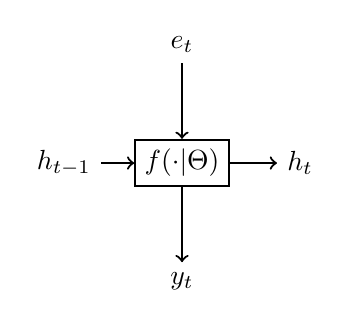
\begin{tikzpicture}[node distance=1.5cm, auto, thick]
        % Nodes
        \node (f) [draw, rectangle] {$f(\cdot|\Theta)$};
        \node (h_old) [left of=f] {$h_{t-1}$};
        \node (e) [above of=f] {$e_t$};
        \node (h) [right of=f] {$h_t$};
        \node (y) [below of=f] {$y_t$};

        % Edges
        \draw[->] (h_old) -- (f);
        \draw[->] (e) -- (f);
        \draw[->] (f) -- (h);
        \draw[->] (f) -- (y);
    \end{tikzpicture}
    \caption{RNN cell}
    \label{fig:rnn_cell}
\end{figure}

The RNN is a parametrized learnable function $f(\cdot|\Theta)$ s.t.
\[
    f(e_t,h_{t-1}|\Theta): \mathbb{R}^{1\times d}\times\mathbb{R}^{1\times h}\rightarrow\mathbb{R}^{1\times h}\times\mathbb{R}^{1\times m}
\]

$f$ is called the \textbf{RNN cell}.

Given a RNN cell, a sequence of $n$ words $w_1,\dots,w_n$ and their embeddings $e_1,\dots,e_n$ and $h_0=0$
we can compute the hidden states and the output of the model as follows:
\[
    h_t,y_t=f(e_t,h_{t-1}|\Theta)
\]

\begin{figure}[H]
    \centering
    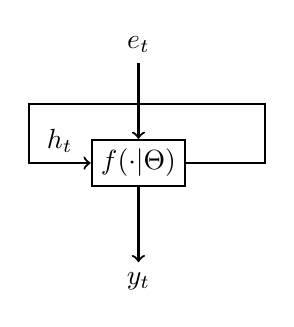
\begin{tikzpicture}[node distance=1.5cm, auto, thick]
        % Nodes
        \node (f) [draw, rectangle] {$f(\cdot|\Theta)$};
        \node (e) [above of=f] {$e_t$};
        \node (y) [below of=f] {$y_t$};

        % Edges
        \draw[->] (e) -- (f);
        \draw[->] (f) -- (y);
        \draw[->] (f.east) -- +(1,0) -- +(1,0.75) -- +(-2,0.75) -- +(-2,0) -- (f.west) node[above, pos=0.5] {$h_t$};
    \end{tikzpicture}
    \caption{RNN model}
    \label{fig:rnn_model}
\end{figure}

The input of our RNN model is a sequence of words $w_1,\dots,w_n$. The words are converted to embeddings $e_1,\dots,e_n$ 
using an embedding matrix $E$.
The output ($y_i$) of each cell is $P[w_{i+1}|h_i]$.
The simplest kind of cell is the linear cell (it's not used anymore).

\begin{figure}[H]
    \centering
    \begin{tikzpicture}[node distance=1.5cm, auto, thick]
        % Nodes
        \node (h_old) [] {$h_{t-1}$};
        \node (e) [below of=h_old] {$e_t$};
        \node (Whh) [draw, trapezium, shape border rotate=270, right of=h_old] {$W_{hh}$};
        \node (Weh) [draw, trapezium, shape border rotate=270, right of=e] {$W_{eh}$};
        \node (sum) [draw, circle, right of=Whh] {$+$};
        \node (sigma) [draw, rectangle, right of=sum] {$\sigma$};
        \node (Why) [draw, trapezium, shape border rotate=90, below of=sigma] {$W_{hy}$};
        \node (softmax) [draw, rectangle, right of=Why, rotate=90] {softmax};
        \node (y) [right of=softmax] {$y_t$};
        \node (h) [right of=sigma] {$h_t$};

        % Edges
        \draw[->] (h_old) -- (Whh);
        \draw[->] (e) -- (Weh);
        \draw[->] (Whh) -- (sum);
        \draw[->] (Weh) -| (sum);
        \draw[->] (sum) -- (sigma);
        \draw[->] (sigma.east) -- ++(0.5,0) -- ++(0,-0.5) -- ++(-1.5,0) |- (Why.west);
        \draw[->] (Why) -- (softmax);
        \draw[->] (softmax) -- (y);
        \draw[->] (sigma) -- (h);
    \end{tikzpicture}
    \caption{Linear RNN cell}
    \label{fig:linear_rnn_cell}
\end{figure}

The weights of the model are of size
\begin{itemize}
    \item $W_{hh}\in\mathbb{R}^{h\times h}$ (hidden to hidden)
    \item $W_{eh}\in\mathbb{R}^{d\times h}$ (embedding to hidden)
    \item $W_{hy}\in\mathbb{R}^{h\times |V|}$ (hidden to output)
\end{itemize}

The first major problem is that to compute the hidden state $h_t$ we need to compute $h_{t-1}$.
There is also a problem with the gradients of the loss.
When we do the backpropagation, the gradients flow trough all the cells
until they reach $h_0$.
Also the backpropagation \textbf{through time} is very slow because
it's as sequential as the forward pass.

Let's call all the parameters of the model $W$.
The loss of the model is:
\[
    \mathcal{L}_t(W)=log(P[w_{t+1}|w_1,\dots,w_t])
\]

The gradient is
\[
    \frac{\partial \mathcal{L}}{\partial W}
    =-\frac{1}{|T|}\sum_{t=1}^{|T|}\frac{\partial \mathcal{L}_t}{\partial W}
    =-\frac{1}{|T|}\sum_{t=1}^{|T|}\frac{\partial \mathcal{L}_t}{\partial y_t}\frac{\partial y_t}{\partial h_t}\frac{\partial h_t}{\partial W}
\]

The problem is that $h_t$ depends on $h_{t-1}$ and so on.
To be precise $h_t=f(x_t,h_{t-1}|W)$.
So the derivative of $h_t$ with respect to $W$ is
\[
    \frac{\partial h_t}{\partial W}=\sum_{k=0}^{t-1}\frac{\partial h_t}{\partial h_k}\frac{\partial h_k}{\partial W}
\]
\[
    \frac{\partial h_t}{\partial h_k}=\prod_{j=k+1}^t\frac{\partial h_j}{\partial h_{j-1}}
\]

So the gradient of the loss with respect to $W$ is
\[
    \frac{\partial \mathcal{L}}{\partial W}
    =-\frac{1}{|T|}\sum_{t=1}^{|T|}\frac{\partial \mathcal{L}_t}{\partial y_t}\frac{\partial y_t}{\partial h_t}\sum_{k=0}^{t-1}\prod_{j=k+1}^t\frac{\partial h_j}{\partial h_{j-1}}\frac{\partial h_k}{\partial W}
\]
We compute explicitly the derivative of $h_j$ with respect to $h_{j-1}$:
\[
    \frac{\partial h_j}{\partial h_{j-1}}=\frac{\partial\sigma}{\partial h_{j-1}}W^T
\]

The magnitude of the gradient of $h_j$ w.r.t. $h_{j-1}$ is composed of:
\begin{itemize}
    \item The derivative of the activation function $\sigma$.
    It's upper bounded by $\beta_\sigma$.
    \item The matrix $W^T$. It's upper bounded by $\beta_W$.
\end{itemize}

So the derivative $\frac{\partial h_t}{\partial h_k}$ (the big product) is upper bounded by
\[
    \left|\prod_{j=k+1}^t\frac{\partial h_j}{\partial h_{j-1}}\right| \leq \left(\beta_\sigma\beta_W\right)^{t-k}
\]

The bound is exponential in the distance between $t$ and $k$.
When $t$ becomes large, if $\beta_\sigma\beta_W<1$ the gradient of the 
first cells will be almost zero (\textbf{vanishing gradient}).
If $\beta_\sigma\beta_W>1$ the gradient will be near infinity (\textbf{exploding gradient}).

The longer the sequence, the more the gradient will be affected by this problem.
There is a technique called \textbf{gradient clipping} that can help with the exploding gradient problem
but there's no solution for the vanishing gradient problem.

\subsubsection{Seq2Seq models}
\label{sec:seq2seq_models}

When we want to take a sequence as input and output a new sequence like in machine translation,
we need a new kind of model called \textbf{sequence-to-sequence} model.
This model is also called \textbf{encoder-decoder} model.

A first network called \textbf{encoder} reads the input sequence and produces a fixed-size representation of it (\textbf{state}).
This state is also called \textbf{context}.
Then a second network called \textbf{decoder} reads the context and produces the output sequence.

\begin{figure}[H]
    \centering
    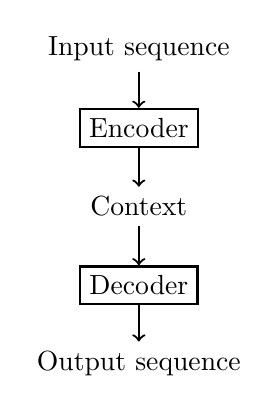
\begin{tikzpicture}[node distance=1cm, auto, thick]
        % Nodes
        \node (input) {Input sequence};
        \node (encoder) [draw, rectangle, below of=input] {Encoder};
        \node (context) [below of=encoder] {Context};
        \node (decoder) [draw, rectangle, below of=context] {Decoder};
        \node (output) [below of=decoder] {Output sequence};

        % Edges
        \draw[->] (input) -- (encoder);
        \draw[->] (encoder) -- (context);
        \draw[->] (context) -- (decoder);
        \draw[->] (decoder) -- (output);
    \end{tikzpicture}
    \caption{Encoder-Decoder model}
    \label{fig:encoder_decoder}
\end{figure}

An implementation with RNNs is the following:

\begin{figure}[H]
    \centering
    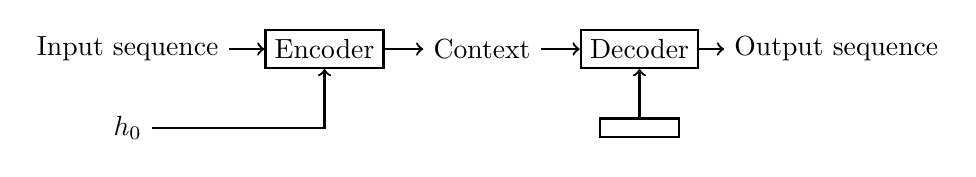
\begin{tikzpicture}[node distance=1cm, auto, thick]
        % Nodes
        \node (input) {Input sequence};
        \node (h_0) [below of=input] {$h_0$};
        \node (encoder) [draw, rectangle, right of=input, node distance=2.5cm] {Encoder};
        \node (context) [right of=encoder, node distance=2cm] {Context};
        \node (decoder) [draw, rectangle, right of=context, node distance=2cm] {Decoder};
        \node (ground) [draw, rectangle, below of=decoder, minimum width=1cm] {};
        \node (output) [right of=decoder, node distance=2.5cm] {Output sequence};

        % Edges
        \draw[->] (input) -- (encoder);
        \draw[->] (h_0) -| (encoder);
        \draw[->] (encoder) -- (context);
        \draw[->] (context) -- (decoder);
        \draw[->] (decoder) -- (output);
        \draw[->] (ground) -- (decoder);
    \end{tikzpicture}
    \caption{RNN Encoder-Decoder model}
    \label{fig:rnn_encoder_decoder}
\end{figure}

The greedy approach was to generate the output sentence word by word, selecting at each step the one with the maximum probability.
When we get the end-of-sentence token, we stop.
The problem with this model is that the probability at each step
depends on the selections we made at the previous steps.

This problem can be described like this:
\begin{itemize}
    \item Given an input sentence $S_0$
    \item Given a language model $P(s)$
\end{itemize}
The problem is $\text{argmax}_{S\in V^+}log P(s|S_0) = S^*$
Unfortunately, the problem requires an exhaustive search over all the possible sentences.

How can we solve this problem?
The first solution is to use a \textbf{beam search}.
The beam search doesn't select a single path. Let's call a traversal of the tree
a \textbf{beam}. At each step, the beam search selects the $k$ most probable beams.
Then we expand them to the next token and select again the $k$ most probable beams.
We stop when each beam has the end-of-sentence token.
Then we select the most probable beam.

A different approach is to use a \textbf{random search}.
At each step select with probability $P[w_i|w_{i-1},\dots,w_1]$ the next word.
We use only the top-$k$ most probable words.

Another option is to use \textbf{temperature}.
The temperature is a parameter that can be used to control the probability distribution
in the softmax function.
The temperature is a positive number that is used in the softmax exponential function.
\[
    e^{x_i/T}
\]
The temperature will be used in combination with the other techniques to make the sentence more interesting.
